\documentclass[12pt]{book}

%= Set Thai Language ==================================
%= ใช้ XeLaTeX

\usepackage[vcentering,dvips]{geometry}
\usepackage{subfigure}
\geometry{papersize={7in,9in},total={4.8in,6.8in}}

\usepackage{pst-tree}
\usepackage{xltxtra}
\usepackage{fontspec}
\usepackage{xunicode}
\usepackage{amsmath}
\usepackage{graphicx}

\XeTeXlinebreaklocale “th_TH” % สำหรับตัดคำ
\XeTeXlinebreakskip = 0pt plus 1pt %
\renewcommand{\baselinestretch}{1.2} % ตั้งระยะห่างระหว่างบรรทัด
\defaultfontfeatures{Scale=1.23}

%\newfontfamily{\thaifont}[Script=Thai]{TH Sarabun New:script=thai}

\setromanfont[
BoldFont=THSarabun_Bold.ttf,
ItalicFont=THSarabun_Italic.ttf,
BoldItalicFont=THSarabun_Bold_Italic.ttf,
]{THSarabun.ttf}


%\setmainfont[Script=Thai]{THSarabunNew.ttf}

\renewcommand{\figurename}{รูปที่}
\renewcommand{\chaptername}{บทที่}

\newcounter{examplecounter}
\newenvironment{example}{%
  \refstepcounter{examplecounter}%
  \textbf{ตัวอย่างปัญหา \thechapter-\arabic{examplecounter}}%
}{%
}

% =====================================================

\begin{document}

\title{\textbf{ความซับซ้อนของปัญหาและกระบวนการแก้ปัญหาโดยวิธีประมาณ}}
% Include Author name and Copyright holder name
\author{ผู้ช่วยศาสตราจารย์ ดร.พงศ์พันธ์ กิจสนาโยธิน}

\chapter{บทนำ}

\par{
ก่อนจะถึงในรายละเอียดข้างต้น 
ในส่วนแรกจะกล่าวถึงประวัติและความเป็นมาของ
ระบบการคำนวณอันเป็นที่มาของสถาปัตยกรรมคอมพิวเตอร์
}

\par{
Charles Babbage เป็นศาสตราจารย์ในสาขาคณิตศาสตร์ที่มหาวิทยาลัย 
Cambridge ในช่วง 1827 ถึง 1839 ซึ่งถูกยกย่องว่า
เป็นบิดาแห่งคอมพิวเตอร์ (father of the computer) 
\cite{halacy1970charles}
เนื่องจากเป็นผู้คิดค้นเครื่องคำนวณแบบจักรกลเป็นผลสำเร็จเป็นคนแรก อัน
นำมาซึ่งในการออกแบบเครื่องคำนวณในรูปแบบต่าง ๆ ที่มีความซับซ้อนมากยิ่งขึ้น 
หนึ่งในเครื่องจักรการคำนวณที่จะกล่าวถึงคือ Different Engine 
(ถูกออกแบบในปี 1823) ดังแสดงในรูปที่ 
\ref{fig_babbage_difference_engine}
}
%
%
\begin{figure}[h]
\centering
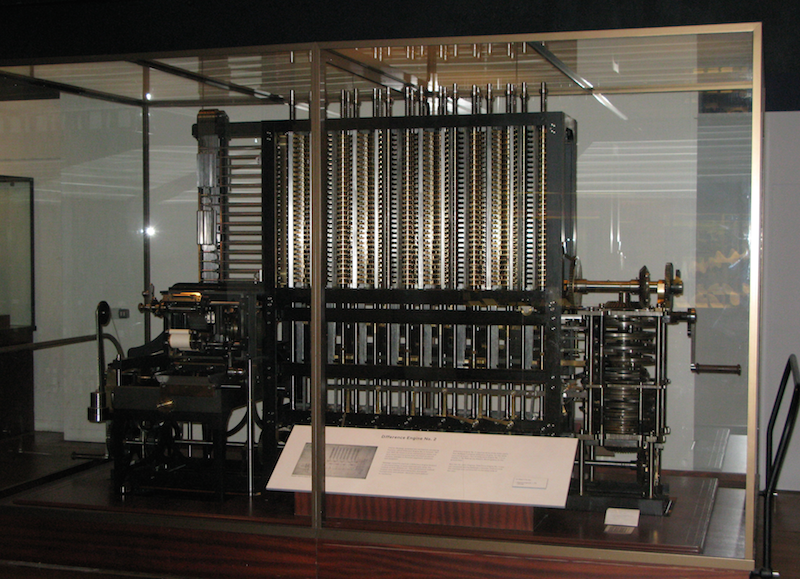
\includegraphics[width=0.75\textwidth]{fig/Babbage_Difference_Engine.png}
\caption{Different Engine ที่ถูกจัดแสดงใน London Science Museum}
\label{fig_babbage_difference_engine}
\end{figure}
%
%
\par{
จุดมุ่งหมายของการออกแบบ Different Engine 
คือต้องการใช้เครื่องจักรในการแก้ปัญหาทางคณิตศาสตร์ที่มีหลัก
ในการแก้เป็นแบบการวนซ้ำ (Iteration) ซึ่งปัญหาคณิตศาสตร์
ดังกล่าวคือ การหาค่าของสมการพหุนามด้วย 
Finite Difference Method ตัวอย่างเช่น  
กำหนดให้  $f(x) เป็นฟังก์ชั่นพหุนาม โดยที่มีค่าเป็น 
$x^2 + x + 33$ ดังนั้น
%
\begin{align}
f(x)&=x^2+x+33\\
d_1(x)&=f(x) - f(x-1) = 2x\\
d_2(x)&=d_1(x) - d_1(x-1) = 2
\end{align}
%
ในทางย้อนกลับจากข้างต้นจะได้ว่า
%
\begin{align}
d_2(x)&=2\\
d_1(x)&=d_1(x-1) + d_2(x) \\
f(x)&=f(x-1) + d_1(x)
\end{align}
%
จากชุดของสมการข้างต้นสามารถสร้างตาราง
ในการคำนวณค่าของพหุนามสำหรับค่าที่กำหนดให้ 
$x$ ใด ๆ ดังแสดงในตารางที่ 
\ref{tab:finite_difference_method}
%
\begin{table}
\caption{ตัวอย่างปัญหาที่แก้ด้วยวิธี Finite Difference Method}
\label{tab:finite_difference_method}
\begin{center}
\begin{tabular}{|l|c|c|c|c|c|c|c|}
$x$ & 0 & 1 & 2 & 3 & 4 & 5 & 6 \\
\hline
$d_2(x) & & & 2 & 2 & 2 & 2 & 2 \\
$d_1(x) & & 2 & 4 & 6 & 8 & 10 & 12 \\
$f(x) & 33 & 35 & 39 & 45 & 53 & 63 & 75 
\hline
\end{tabular}
\end{center}
\end{table}
%
กรณีที่ต้องการหาค่าของ $f(x)$ 
เมื่อ $x$ มีค่าเป็น 3 สามารถคำนวณได้จาก 
ค่าของ $f(2)$ และ $d_1(2)$ ดังนี้ 
%
\begin{align}
d_2(3)&=2\\
d_1(3)&=d_1(2) + d_2(3) \\
&= 4 + 2 = 6 \\
f(3)&=f(2) + d_1(3) \\
&= 39 + 6 = 45
\end{align}
%
จะเห็นได้ว่าการคำนวณหาของพหุนามนั้นเป็นการ
ท ำบวกซ้ำ ๆ กันของค่าที่คำนวณก่อนหน้า 
ซึ่งเป็นพื้นฐานในการแก้ปัญหาด้วยวิธีการวนซ้ำ 
การออกแบบเครื่องจักรกล Different Engine ของ 
Babbage สามารถสร้างขึ้นและทำงานได้จริงในปี 1855 
โดย Scheutz โดยเครื่องจักรดังกล่าว 
สามารถคำนวณพหุนามได้ถึงดีกรีที่ 6 
}


%\chapter{NP-Completeness}

\par{
NP-Completeness เป็นเรื่องที่เราต้องการจะแสดงให้เห็นว่า 
ปัญหาที่เราต้องการจะแก้นั้นยากแค่ไหน 
ซึ่งเราไม่สามารถหา วิธีการแก้ที่มีประสิทธิภาพมาแก้ปัญหานั้น ๆ ได้ 
ทดสอบการแก้ไข
}

\par{
ปัญหา คือ ความสัมพันธ์ทวิภาค (binary relation) ระหว่าง เซตตัวแสดงลักษณะของปัญหา $I$ (instances) ไปยัง เซตของ คำตอบของปัญหา (solutions) $S$ ตัวอย่างเช่น ปัญหาการหาเส้นทางระหว่างจุดยอดสองจุดในกราฟ เป็นความสัมพันธ์ทวิภาค ของเซตของตัวแสดงลักษณะของปัญหา $\left<G, u, v\right> \in I$ โดยที่ $G$ เป็นกราฟ $u$ และ $v$ เป็นสองจุดยอดในกราฟ $G$ ไปยังเซตของ คำตอบของปัญหา $p \in S$ เป็น ลำดับของจุดยอดจากจุดยอด $u$ เป็นยัง $v$ หรือ เป็นลำดับที่ไม่มีสมาชิก ($p = \left<\right>$) ในกรณีที่ไม่มีเส้นทางจากจุดยอด $u$ ไปยัง $v$ 
}

\par{
ลักษณะของการอธิบายปัญหาในข้างต้นเป็นรูปแบบทั่วไป ตัวอย่างหนึ่งของปัญหาที่มีลักษณะเฉพาะคือ ปัญหาแบบการหาค่าที่ดีที่สุด (Optimization problem) ซึ่งคำตอบของปัญหาในลักษณะนี้ จะมีค่าที่น้อยที่สุดหรือมากที่สุดขึ้นอยู่กับคำถามของปัญหา ตัวอย่างเช่น ปัญหาการหาเส้นทางที่สั้นที่สุดระหว่างจุดยอดสองจุดในกราฟ ซึ่งจะเห็นได้ว่า ตัวแสดงลักษณะของปัญหา จะเหมือนกันกับ ปัญหาการหาเส้นทางระหว่างจุดยอดสองจุดในกราฟ ($\left<G, u, v\right>$) แต่ คำตอบของปัญหานี้ จะแสดงเฉพาะเส้นทางที่มีระยะทางน้อยที่สุดเท่านั้น
}

\par{
นอกจาก ปัญหาแบบการหาค่าที่ดีที่สุด แล้วยังมีปัญหาลักษณะเฉพาะแบบ ตัดสินใจ (Decision problem) ซึ่งจะมีลักษณะของคำตอบของปัญหาเป็น ใช่ หรือ ไม่ใช่ จากตัวอย่างของ ปัญหาการหาเส้นทางที่สั้นที่สุด เราสามารถเปลี่ยนให้ลักษณะของปัญหาให้เป็นแบบตัดสินใจ โดยการระบุค่าคงที่ของ ระยะทางระหว่าง สองจุดยอด ซึ่งจะเป็นปัญหาใหม่ คือ ปัญหาการตรวจสอบว่ามีเส้นทางระหว่างจุดยอดสองจุด $u$ และ $v$ ในกราฟ $G$ ที่มีระยะห่างไม่เกินค่าคงที่ $k$ ฉะนั้น ตัวแสดงลักษณะของปัญหาการตรวจสอบนี้ คือ $\left<G, u, v, k\right>$ และ คำตอบของปัญหาจะเป็น ใช่ ถ้ามีเส้นทางระยะน้อยกว่าหรือเท่ากับ $k$ จากจุดยอด $u$ ไป $v$ หรือ ไม่ใช่ ถ้าไม่มีเส้นทางจาก $u$ ไป $v$ ที่มีระยะน้อยกว่าหรือเท่ากับ $k$ ในบทนี้เราจะเน้นการศึกษาในลักษณะของปัญหาแบบ ตัดสินใจ เพื่อความเข้าใจที่ง่ายขึ้นเราจะใช้ ทฤษฎีภาษารูปนัย (Formal-language theory) อธิบายลักษณะของปัญหาประเภทนี้ 
}

\par{
กำหนดให้ $\Sigma$ เป็น เซตที่มีจำนวนจำกัดของตัวอักขระ ภาษา $L$ ที่เกิดขึ้นจาก $\Sigma$ คือ เซตของคำ (strings) ใด ๆ ก็ตามที่ประกอบขึ้นด้วยการนำตัวอักขระจาก $\Sigma$ มารวมกัน ตัวอย่างเช่น ถ้า $\Sigma$ เป็น เซตของตัวอักขระ 0 และ 1 ($\Sigma = \{0, 1\}$) ภาษา $L$ ซึ่งประกอบด้วยตัวเลขฐานสองที่แสดงค่าเป็นจำนวนเฉพาะจะเป็น เซตต่อไปนี้ $\{10, 11, 101, 111,$ $1011, 10001, \ldots \}$
} 

\par{
ภาษา $B$ เป็น NP-complete ก็ต่อเมื่อ (1) ภาษา $B$ เป็น NP และ (2)
ทุก ๆ ภาษา $A$ ที่เป็น NP สามารถเปลี่ยนให้เป็นภาษา $B$ โดยใช้เวลาเป็นโพลิโนเมียล
}

\par{
เพื่อความง่ายในการจะพิสูจน์ว่า ภาษาหนึ่ง ๆ จะเป็น NP-complete หรือไม่นั้น เราจำเป็นต้องหา ปัญหาแรกที่เราทราบว่าเป็น NP-complete จากนั้นเราจะหากระบวนการแปลงที่ใช้เวลาเป็นโพลิโนเมียลเพื่อ แปลงจากปัญหาแรกเป็นปัญหาที่เราต้องการจะพิสูจน์แทนที่จะพิสูจน์ว่า ภาษานั้น ๆ เป็น NP-complete โดยตรง ซึ่งเราจะเลือก SAT เป็นปัญหาแรกที่เราจะพิสูจน์ว่าเป็น NP-complete
}

\section{The Cook-Levin Theorem}

\par{เนื้อหาในส่วนนี้เราจะทำความเข้าใจเกี่ยวกับ Cook-Levin Theorem ซึ่งเป็นการพิสูจน์ว่า SAT เป็น NP-complete problem}

\par{
การจะพิสูจน์ SAT เป็น NP-complete เราจำเป็นต้องพิสูจน์ว่า SAT เป็น NP และทุก ๆ NP สามารถเปลี่ยนให้เป็น SAT โดยกระบวนการที่ใช้เวลาเป็นโพลิโนเมียลตามขนาดของปัญหาของ NP นั้น ๆ 
}

\par{
ในการพิสูจน์ว่า SAT เป็น NP นั้น เราสามารถอธิบายได้ว่าเราสามารถใช้ เครื่องจักรแบบเชิงไม่กำหนดซึ่งใช้เวลาในรูปของสมการพหุนาม (Nondeterministic polynomial time machine) ที่สามารถจะคาดเดาการกำหนดค่าของตัวแปรในลอจิก $\phi$ ซึ่งจะยอมรับ (accept) ถ้า การกำหนดค่านั้นทำให้ $\phi$ มีค่าความจริงเป็นจริง ซึ่งเวลาที่ใช้ในการตรวจสอบค่าความจริงของ $\phi$ นั้นจะขึ้นอยู่กับจำนวนตัวแปรที่ปรากฏอยู่ใน $phi$ ถ้ากำหนดให้ $n$ เป็น จำนวนตัวแปรใน $\phi$ แล้วเราจะได้ $p(n)$ ซึ่งเป็นฟังก์ชันพหุนามแสดงเวลาที่ใช้สำหรับการตรวจสอบค่าความจริงของ $\phi$ ($p(n) = O(n^k)$ โดยที่ $k$ เป็นค่าคงที่ค่าหนึ่ง)
}

\par{
ต่อมาเราจะเริ่มพิสูจน์ว่าทุก ๆ ปัญหา $A$ ที่เป็น NP เราสามารถเปลี่ยนให้เป็นปัญหา SAT ได้ เราจะเริ่มต้นโดย กำหนดให้ $N$ เป็น เครื่องจักรทัวร์ลิ่งแบบเชิงไม่กำหนด (Nondeterministic Turing machine) ซึ่งสามารถตัดสินปัญหา $A$ ได้ในเวลา $p(n)$ โดยที่ $p(n)$ เป็นสมการเชิงพหุนาม
}

\par{
หลักการในการพิสูจน์ในกรณีนี้นั้นเราจะต้องเปลี่ยน $N$ ให้กลายเป็นลอจิก $\phi$ โดยที่ถ้า $w \in L$ เป็นอินพุทของ $N$ และ $N$ ยอมรับ $w$ แล้ว $\phi$ ต้องมีค่าความจริงเป็นจริง 
}

\par{
พิจารณาข้อจำกัดแรกของ $N$ กล่าวคือ ณ เวลาใดก็ตามสถานะของ $N$ จะต้องอยู่ใน state ใด state หนึ่งเท่านั้น จากข้อจำกัดนี้ เราจะนิยาม ตัวแปร logic $Q_{ij}$ เป็นตัวบอกว่า $N$ อยู่ ณ state $i$ในเวลาที่ $j$ ถ้า $Q_{ij}$ มีค่าความจริงเป็นจริง เนื่องจากการทำงานของ $N$ จะต้องเสร็จภายใน $p(n)$ แสดงว่า $0 \ge j \le p(n)$ ฉะนั้น เราจะต้องแสดงเป็นลอจิกโดยการใช้ $Q_{ij}$ ให้ได้ว่า ณ เวลาใดก็ตาม $N$ ต้องอยู่ใน state ใด state หนึ่งเท่านั้น
}

\par{
ถ้ากำหนดให้ $N$ มีจำนวน state ทั้งหมด $m$ ฉะนั้น
%
\begin{eqnarray*}
Q_{0j} \vee Q_{1j} \vee \ldots \vee Q_{mj}
\end{eqnarray*}
%
ถ้าค่าของความจริงประโยคข้างต้นเป็นจริงแสดงว่า $N$ ต้องอยู่ใน state ใด state หนึ่ง (หรือมากกว่าหนึ่ง state) ณ เวลาที่ $j$ สำหรับ $0 \ge j \le p(n)$
}

\par{
เนื่องจาก ลอจิกข้างต้นยังไม่ได้ระบุข้อจำกัดเกี่ยวกับ $N$ ต้องอยู่ที่ state เดี่ยวเท่านั้นเราจำเป็นต้องเพิ่มลอจิกต่อไปนี้เพื่อจำกัดว่าต้องเป็น state เดี่ยวเข้าไป ดังต่อไปนี้
%
\begin{eqnarray*}
\neg Q_{pj} \vee \neg Q_{qj} 
\end{eqnarray*}
%
สำหรับค่า $p$, $q$ ใด ๆ ก็ตามที่มากกว่า 0 แต่น้อยกว่า m (เนื่องจากเรามี state ทั้งหมด $m$) โดยที่ $p$ และ $q$ มีค่าไม่เท่ากัน
}

\par{
จากการทำงานของ $N$ ที่ต้องใช้เวลาเป็น $p(n)$ สำหรับอินพุท $w$ เราสร้าง ตัวแปรลอจิก $Q_{ij}$ ขึ้นมา โดยมี logic statement ทั้งหมด  

\begin{itemize}
\item $p(n)$  สำหรับ $Q_{0j} \vee Q_{1j} \vee \ldots \vee Q_{mj}$
\item $p(n)\frac{m(m-1)}{2}$ สำหรับ $\neg Q_{pj} \vee \neg Q_{qj}$ 
\end{itemize}

จะเห็นได้ว่า การสร้าง logic statement สำหรับ แสดงการทำงานของ $N$ ในกรณีนี้เป็น พหุนามของ $p(n)$ ถ้ากำหนดให้ $m$ เป็นค่าคงที่
}

\par{
พิจารณาข้อจำกัดต่อมาของ $N$ คือ ณ เวลาใด ๆ หัวอ่านเขียนของ $N$ จะต้องอยู่ที่ตำแหน่งใดตำแหน่งหนึ่งของแถบการทำงานของ $N$ ตำแหน่งเดี่ยวเท่านั้น
}

\par{
เช่นเดียวกันกับ $Q_{ij}$ เราจะกำหนด $P_{ij}$ เพื่อแสดงตำแหน่งว่าหัวอ่านเขียนของ $N$ ณ เวลา $j$ อยู่ที่ตำแหน่ง $i$ ฉะนั้นเราจะได้ว่า
%
\begin{eqnarray*}
P_{0j} \vee P_{1j} \vee \ldots \vee P_{mj} 
\end{eqnarray*}
%
ในกรณีนี้เนื่องจาก $N$ ต้องทำงานเสร็จในเวลา $p(n)$ ความยาวของแถบต้องมีค่าไม่เกิน $p(n)$ ถ้าเราสมมุติให้การเคลื่อนของหัวอ่านเขียนหนึ่งครั้งแทนการใช้เวลาหนึ่งหน่วย ฉะนั้นค่าของ $m$ จึงต้องมีค่า $0 \ge m \le p(n)$ เช่นเดียวกันกับค่าของ $0 \ge j \le p(n)$ 
}

\par{
ในเวลาใด ๆ หัวอ่านต้องอยู่ที่ตำแหน่งเดี่ยวเท่านั้น สามารถแสดงเป็น Logic statement เพิ่มเติมจากตัวบนได้ดังต่อไปนี้
%
\begin{eqnarray*}
\neg P_{pj} \vee \neg P_{qj} 
\end{eqnarray*}
%
โดยที่ $p$ และ $q$ ไม่เท่ากันและมีค่า $0 \ge p, q \le p(n)$ โดยสรุปการสร้าง logic statement สำหรับตำแหน่งหัวอ่านเขียนของ $N$ นั้นจะมีทั้งสิ้น $p(n) + \frac{p(n)(p(n)-1)}{2}$ ซึ่งประมาณได้เป็น $p(n)^2$ 
}

\par{
ข้อจำกัดต่อมาของ $N$ ที่เราต้องคำนึงถึงคือ ค่าในแถบข้อมูลในแต่ละช่องต้องมีได้แค่ค่าเดี่ยวเท่านั้น เริ่มด้วยกำหนดให้ $S_{ijk}$ เป็นตัวแปรลอจิก เพื่อแสดงว่า ณ เวลา $k$ มีค่า $j$ ตรงตำแหน่งแถบที่ $i$ ฉะนั้น
%
\begin{eqnarray*}
S_{i0k} \vee S_{i1j} \vee \ldots \vee S_{ivj} 
\end{eqnarray*}
%
จะมีค่าความจริงเป็นจริงเพื่อแสดงให้เห็นว่า อย่างน้อยในเวลา $j$ ใด ๆ ณ ตำแหน่งแถบที่ $i$ จะต้องมีค่าอย่างน้อยหนึ่งค่าเสมอ จำนวนลอจิกข้างต้นคิดเป็น $p(n)^2$ โดยที่ $0 \ge i, j \le p(n)$ และ $v$ เป็นค่าคงที่  
}

\par{
ต่อมาเราต้องระบุด้วย logic statement เพื่อจำกัดว่าต้องมีแค่ค่าเดี่ยวเท่านั้น ด้วย
%
\begin{eqnarray*}
\neg S_{ipj} \vee \neg P_{iqj} 
\end{eqnarray*}
%
โดยที่ $p$ ไม่เท่ากับ $q$ สำหรับ $i$ และ $j$ ใด ๆ ซึ่ง logic statement นี้จะมีจำนวนทั้งสิ้น $p(n)^2\frac{v(v+1)}{2}$
}

\par{
ทั้งสามข้อกำจัดข้างต้นเป็นการบอกสถานะต่าง ๆ ของ state ของ $N$ ตำแหน่งของหัวอ่านเชียน และ ค่าของตำแหน่งในแถบ ตามลำดับ ต่อมาเราจะพิจารณาข้อจำกัดการเปลี่ยน state ของ $N$ โดยมีอยู่ด้วยกันสองประเภทคือ แถบที่ไม่ได้อยู่ ณ ตำแหน่งหัวอ่านเชียนต้องไม่มีการเปลียนแปลงค่าเมื่อมีการเปลี่ยน state และ แถบที่อยู่ ณ ตำแหน่งหัวอ่านเขียนจะเปลี่ยนไปตามการทำงานที่ระบุไว้ใน $N$
}

\par{
เริ่มต้นด้วย แถบที่ไม่ได้อยู่ ณ ตำแหน่งหัวอ่านเชียนต้องไม่มีการเปลียนแปลงค่าเมื่อมีการเปลี่ยน state ซึ่งสามารถเขียนเป็น logic statement ได้ดังต่อไปนี้
%
\begin{eqnarray*}
\neg P_{ij} \rightarrow (S_{ivj} \rightarrow S_{iv,j+1})
\end{eqnarray*}
%
เปลี่ยนให้เป็นรูปแบบตาม SAT ได้ดังต่อไปนี้
%
\begin{eqnarray*}
P_{ij} \vee \neg S_{ivj} \vee S_{iv,j+1}
\end{eqnarray*}
%
ซึ่งจะมีจำนวนทั้งสิ้น $p(n)^2v$
}


\par{
ในกรณีของ แถบที่อยู่ ณ ตำแหน่งหัวอ่านเขียนจะเปลี่ยนไปตามการทำงานที่ระบุไว้ใน $N$ นั้น ถ้ากำหนดให้การทำงานของ $N$ ณ state $i$ ในกรณีที่ค่าในแถบที่หัวอ่านเขียนอยู่เป็น $p$ นั้น $N$ จะเปลี่ยนเป็น state $j$ โดยที่เปลี่ยนแปลงค่า ณ ตำแหน่งหัวอ่านเขียนเป็น $q$ และ เคลื่อนที่หัวอ่านเขียน $d$ จากตำแหน่งปัจจุบัน (สามารถเขียนเป็นการทำงานได้ดังต่อไปนี้ $(i, p) \rightarrow \left[ j, q, d\right]$)  
}

\par{
เราเริ่มจากกำหนด $Q_{ij}$ $P_{kj}$ และ $S_{kpj}$ มีค่าความจริงเป็นจริง เพื่อแสดงว่า $N$ ทำงาน ณ เวลา $j$ จะอยู่ในstate $i$ หัวอ่านเชียนอยู่ที่ตำแหน่ง $k$ โดยที่ค่าของแถบที่หัวอ่านเขียนอยู่มีค่าเป็น $p$ ฉะนั้นในกรณีที่มีการเปลี่ยนจาก state $i$ เป็น state $j$ ตามข้อกำหนดข้างต้นเราจะได้
%
\begin{eqnarray*}
(Q_{ij} \wedge P_{kj} \wedge S_{kpj}) \rightarrow Q_{j,j+1}
\end{eqnarray*}
%
หรือ
%
\begin{eqnarray*}
\neg Q_{ij} \vee \neg P_{kj} \vee \neg S_{kpj}) \vee Q_{j,j+1}
\end{eqnarray*}
%
ซึ่งจะมีจำนวน logic statement ทั้งสิ้น $m^2p(n)^2v$ 
}

\par{
เช่นเดียวกันสำหรับกรณีที่มีการเปลี่ยนแปลงค่าในแถบข้อมูล เราจะได้
\begin{eqnarray*}
\neg Q_{ij} \vee \neg P_{kj} \vee \neg S_{kpj}) \vee S_{kq,j+1}
\end{eqnarray*}
%
ซึ่งจะมีจำนวน logic statement ทั้งสิ้น $mp(n)^2v^2$ 
}

\par{
และในกรณีสุดท้ายสำหรับการเปลี่ยนแปลง state คือการเคลื่อนที่ของหัวอ่านเขียน เราจะได้
\begin{eqnarray*}
\neg Q_{ij} \vee \neg P_{kj} \vee \neg S_{kpj}) \vee P_{k+d,j+1}
\end{eqnarray*}
%
ซึ่งจะมีจำนวน logic statement ทั้งสิ้น $mp(n)^2v$ จะเห็นได้ว่าทั้งสามกรณีข้างต้น ยังมีจำนวน logic เป็น พหุนามของ $p(n)$ 
}

\par{
ต่อมาเราจะสร้าง logic statement ของ การเริ่มต้นการทำงาน และ สิ้นสุดการทำงานของ $N$ โดยสำหรับกรณีเริ่มต้นการทำงาน เรากำหนดให้ $Q_{00}$ $P_{00}$ มีความค่าจริงเป็นจริง ณ ตอนเริ่มทำงานของ $N$ และ ค่าเริ่มต้นของแถบข้อมูลคือ $S_{ir0}$ มีค่าความจริงเป็นจริง สำหรับข้อมูลที่มีขนาด $n$ โดยที่ $0 \ge i \le n$ และ $r$ เป็น ค่าของอินพุท ณ ตำแหน่ง ​$i$  
}

\par{
ในกรณีสิ้นสุดการทำงาน ถ้ากำหนดให้ state $m$ เป็น accepting state แล้ว ณ ตอนสิ้นสุดการทำงานของ $N$ (ณ เวลา $p(n)$) $N$ จะต้องอยู่ ณ state $m$ ฉะนั้นเราสามารถสร้าง logic statement สำหรับระบุการ accepting ของ $N$ ได้ดังนี้ $Q_{m,p(n)}$
}

\par{
จะเห็นได้ว่าในการเปลี่ยนแปลงการทำงานของ $N$ มาในรูปของ SAT นั้น ถ้า $N$ ทำงานตามข้อจำกัดของ NDTM แล้ว accept SAT ก็จะมีค่าความจริงเป็นจริงด้วย ซึ่งในการเปลี่ยนแปลงจาก $N$ ที่ใช้เวลาในการทำงานเป็น $p(n)$ เป็น SAT นี้ใช้เวลาเป็นพหุนามของ $p(n)$ จึงสรุปได้ว่า SAT เป็น NP-complete 
}

%\chapter{Steiner Tree}

\par{
ในบทนี้เราจะศึกษาคุณสมบัติของ Steiner Tree ปัญหาของการหา
Steiner Tree จากกราฟที่กำหนดให้ 
}

\par{
เพื่อให้เข้าใจในปัญหา Stenier tree เราจะเริ่มด้วยการศึกษาปัญหาที่มีลักษณะคล้ายกันก่อน
นั้นก็คือปัญหาการหาค่าน้อยที่สุดของ Spanning tree (Minimum spanning tree, MST)
}

\par{
กำหนดให้ $G(S, E)$ เป็นกราฟที่ไม่กำหนดทิศทางและมีการเชื่อมโยงกัน (Undirected and
connected graph) โดยมี $S$ และ $E$ เป็นเซตของจุดยอดและเซตของเส้นเชื่อมระหว่างจุดของ
กราฟ $G$ ตามลำดับ Spanning tree ของ G คือ กราฟ $G'(S, E')$ โดยที่ $E' \subseteq E$
และ $G'$ ยังคงเป็น กราฟที่มีการเชื่อมโยงกันเช่นเดิม
}

\par{
ปัญหา Steiner Tree หรือ ปัญหาการหาค่าที่น้อยที่สุดของ Steiner tree นั้นเป็นปัญหาที่มี
ลักษณะคล้ายคลึงกับ ปํญหาการหาค่าน้อยที่่สุดสำหรับ  Spanning tree 
}


\end{document}
